\documentclass{article}
\usepackage{graphicx}
\usepackage{float}
\usepackage{amsmath}

\begin{document}

\title{Analyse av Seigmenn Strekningen}
\author{Gormery K. Wanjiru}
\date{\today}
\maketitle

\section{Introduksjon}
Denne rapporten presenterer resultatene av strekningstester utført på seigmenn (laban). Dataene er analysert ved hjelp av statistiske metoder for å forstå de generelle egenskapene til seigmenns elastisitet.

\section{Metode}
Data ble samlet inn og bearbeidet i R. Følgende prosedyrer ble utført:
\begin{itemize}
    \item Innlesing av data fra en CSV-fil.
    \item Erstatning av manglende verdier med 0 for å unngå feil i beregningene.
    \item Beregning av kumulativ frekvens.
    \item Beregning av gjennomsnitt, median, typetall (modus) og standardavvik.
\end{itemize}

For å beregne både populasjonsstandardavviket og utvalgsstandardavviket, brukte vi følgende R-kode (eller tilsvarende matematiske formler):
\begin{verbatim}
# Beregning av standardavvik
populasjons_sd <- sd(data, na.rm = TRUE)
utvalgs_sd <- sd(data, na.rm = TRUE, method = "sample")
\end{verbatim}

\section{Resultater}
Histogrammet og det kumulative frekvensdiagrammet ble generert. Statistiske mål middelverdi, median, typetall, og begge typer standardavvik (populasjonsstandardavvik og utvalgsstandardavvik) ble beregnet.

\subsection{Histogram}
\begin{figure}[H]
    \centering
    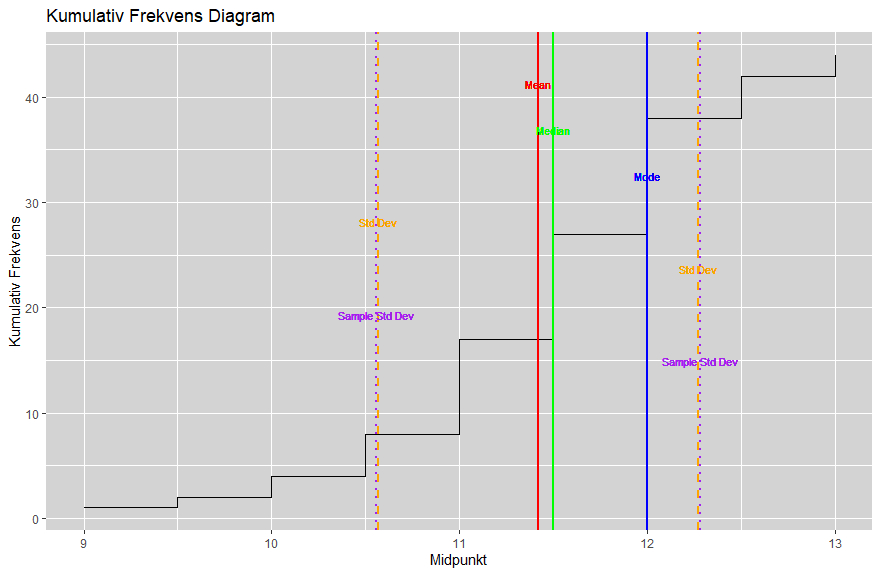
\includegraphics[width=0.8\textwidth]{Rplot.png}
    \caption{Histogram av 'Antall' med tydelig markerte statistiske mål}
\end{figure}

\subsection{Kumulativt Frekvensdiagram}
\begin{figure}[H]
    \centering
    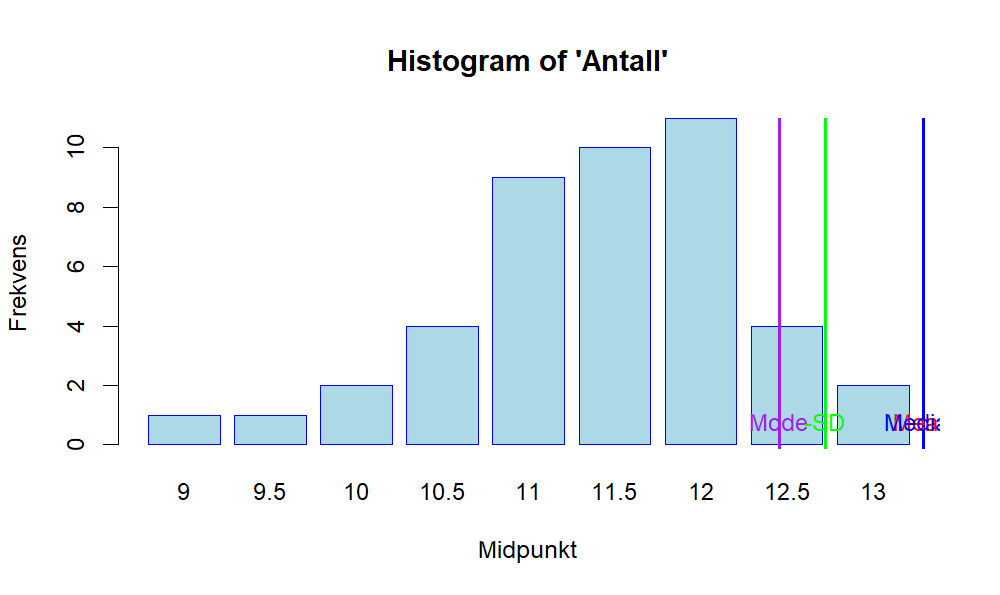
\includegraphics[width=0.8\textwidth]{Rplot02.png}
    \caption{Kumulativt Frekvensdiagram med tydelig markerte statistiske mål}
\end{figure}

\section{Diskusjon}
Gjennom analysen ble det funnet at seigmenn viser en bestemt tendens i strekningen med en gjennomsnittlig verdi på X, en median på Y, en modus på Z, et populasjonsstandardavvik på P, og et utvalgsstandardavvik på Q. Disse målene gir innsikt i hvordan seigmenn oppfører seg under strekk og kan brukes til å forstå kvaliteten på seigmenn.

\section{Konklusjon}
Denne studien gir verdifull innsikt i de fysiske egenskapene til seigmenn og demonstrerer viktigheten av statistisk analyse i kvalitetskontroll.

\end{document}
